\documentclass[11pt]{article}

%%%%%%%%%%%%%%Include Packages%%%%%%%%%%%%%%%%%%%%%%%%%%
\usepackage{xcolor}
\usepackage{mathtools}
\usepackage[a4paper, total={6in, 8in}, margin=1.25in]{geometry}
\usepackage{amsmath}
\usepackage{amssymb}
\usepackage{paralist}
\usepackage{rsfso}
\usepackage{amsthm}
\usepackage{wasysym}
\usepackage[inline]{enumitem}   
\usepackage{hyperref}
\usepackage{tocloft}
\usepackage{titlesec}
\usepackage{colortbl}
%%%%%%%%%%%%%%%%%%%%%%%%%%%%%%%%%%%%%%%%%%%%%%%%%%%%%%%%



\begin{document}
\Large \noindent \textbf{Physics 1A Discussion (Week 1)}\\
\normalsize
Department of Physics and Astronomy, UCLA\\

\noindent TA: Jinyan Miao (PAB 2-429, jnmiu@ucla.edu)\\
Office hour: Monday 4-5 PM at PAB 2-429\\
Tutoring center hour: Monday 10-11 AM over Zoom or at PAB 2-429\\
\noindent\rule{8cm}{0.4pt}\\

\noindent We will start with the TA helping you upload the worksheet to Gradescope. If you are using a paper copy, take a picture of the blank worksheet, convert it to a\ .pdf file and upload it. If you are using an electronic version, simply upload the blank sheet. \\

\noindent During the discussion, you will have time to work on the worksheet. You will overwrite the blank sheet submission at the end of the class. The worksheet will be graded by serious attempt, and is due Tuesday night at 11:59 PM on Gradescope.\\


\hfill\break\hfill\break

\noindent \textbf{Problem 1:} The graph below shows velocity vs.\ time for a motorcycle police officer. \\

\begin{center}
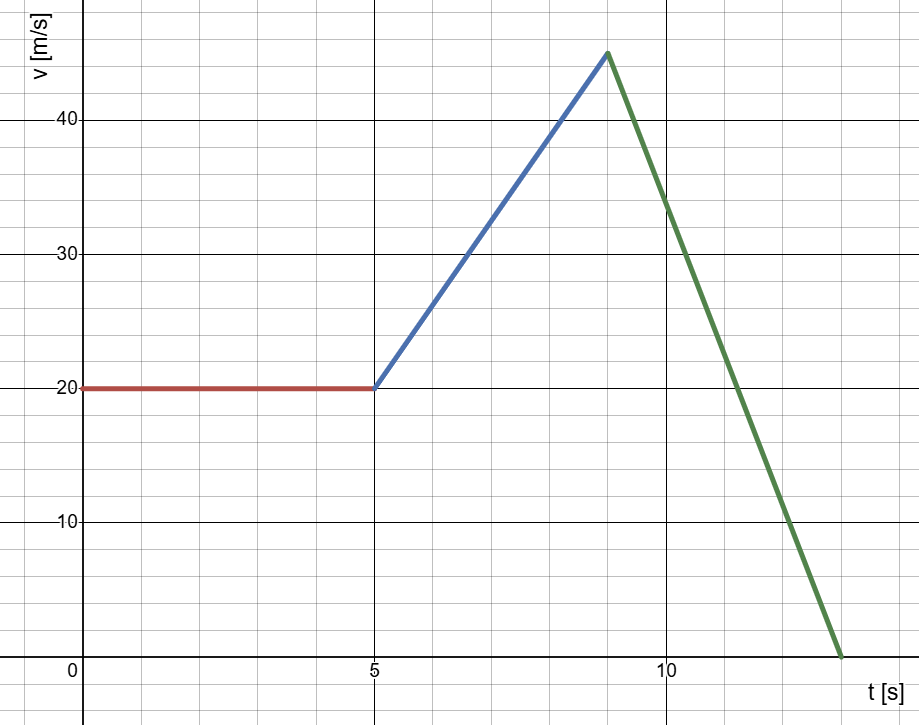
\includegraphics[scale=0.35]{vt}
\end{center}

(a) Find the instantaneous acceleration at time $t=3$\,s, $t=7$\,s, and $t=12$\,s. Then draw the acceleration vs.\ time graph of the officer for the first $13$ seconds. \\

(b) Assuming that the officer starts from the position $x=0$\,m at time $t=0$\,s. Find the position of the officer at $t = 5$\,s, $t=9$\,s, and $t=13$\,s. Draw the position vs.\ time graph of the officer for the first $13$ seconds.\\



\newpage
\textbf{Solutions:}\\

To calculate the acceleration, we look at the slope of the velocity graph. At $t=3$ seconds, slope is zero, so acceleration at $t=3$ seconds is $0$\,m/s$^2$. At $t = 7$\,s, the acceleration is $a = (45-20)/(9-5)=6.25$\,m/s$^2$. At $t=13$\,s, the acceleration is $a=(0-45)/(13-9)=-11.25$ m/s$^2$.\\

To find the position of the police officer, we want to integrate the velocity curve. In this case, since the velocity curve is composed of line segments, we simply look at the area under the curve. At time $t = 5$\,s, the area under the red line is $5\cdot 20=120$ so the position of the police officer is $100$ meters away from the origin. That is, mathematically, 
\begin{align*}
\Delta x _{t=0 \to 5} = \int_0^5 20\, dt = 100\, \text{(meters)}\,.
\end{align*}
At time $t=9\,$s, the total area under the curve is 
\begin{align*}
\Delta x_{t=0\to 9} = \int_0^5 20\, dt + \int_5^9 (\text{blue line})\, dt = 100 + \int_5^9 \left(\frac{25}{4}t -\frac{45}{4}\right)\, dt=230\,(\text{meters}).
\end{align*} 
Thus the police officer is $230$ meters away from the origin. You should also be able to solve it by using the area of small triangles and rectangles bounded by the curves on the graph. At time $t=13$ seconds, we have
\begin{align*}
\Delta x_{t=0\to 13} &= \int_0^5 20\, dt + \int_5^9 (\text{blue line})\, dt+ \int_9^{13} (\text{green line})\, dt \\
&= 100+130 + \int_9^{13} \left(-\frac{45}{4}t +\frac{45}{4}\cdot13\right)\, dt = 230+90 = 320\,(\text{meters})\,.
\end{align*}
We can also do this by calculating the areas of the rectangles and triangles. For instance, at time $t=9$ seconds, we have a rectangle with base $9$ ($\Delta t$) and height $20$, thus a rectangle of area $180$. We also have a triangle with base $9-5=4$ and height $45-20=25$, so a triangle of area $50$. The total area under the curve from $t = 0$ to $t = 9$ is then $180+50=230$, which agrees with what we calculated above.\\

\begin{center}
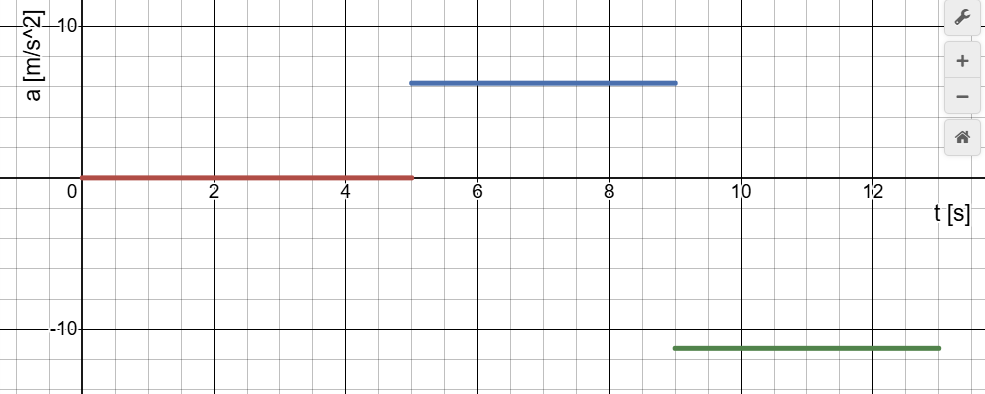
\includegraphics[scale=0.25]{at}
\hfill
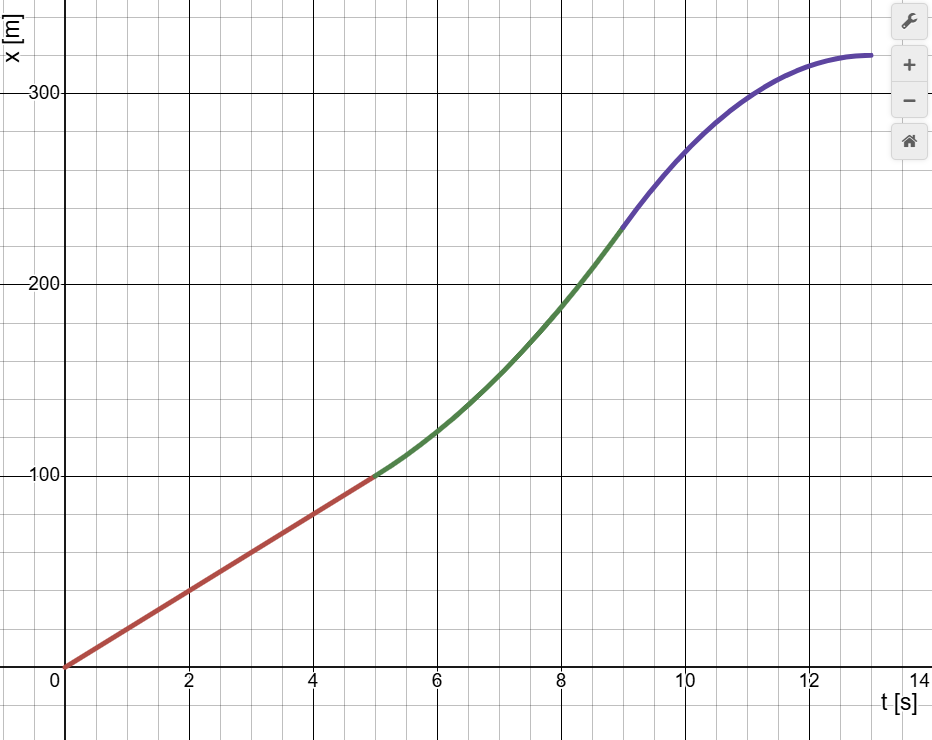
\includegraphics[scale=0.25]{xt}
Acceleration Plot \hfill Position Plot
\end{center}

\end{document}
